\documentclass[11pt]{article}
\usepackage{tocloft}
\usepackage[polish]{babel}
\usepackage[utf8]{inputenc}
\usepackage{float}
\usepackage{enumerate}
\usepackage{listings}
\usepackage{subfig}
\usepackage{graphicx}
\usepackage{mathpazo}
\usepackage[T1]{fontenc}
\usepackage{color}
\usepackage{epstopdf}
\usepackage{amsmath, mathtools}

\usepackage{booktabs}
\usepackage{amsfonts}
\usepackage{amsmath}
\usepackage{tikz}

\usepackage{geometry}
\geometry{verbose,tmargin=2.5cm,bmargin=2.5cm,lmargin=2.5cm,rmargin=2.5cm}

\usepackage[
        unicode=true,
        bookmarks=true,
        bookmarksnumbered=false,
        bookmarksopen=false,
        breaklinks=false,
        pdfborder={0 0 1},
        backref=false,
        colorlinks=false]{hyperref}
		
\hypersetup{
        pdftitle={Impulsowe sieci neuronowe - teoria i zastosowania},
        pdfauthor={Tomasz Pasternak, Karol Olko, Rafał Kułaga, Michał Jędros}}

\linespread{1.15}
\lstloadlanguages{TeX}

\usepackage{titlesec}
\usepackage{titletoc}
\newcommand{\code}[1]{\texttt{#1}}

\begin{document}

\author{Tomasz Pasternak, \\
		Karol Olko, \\
		Rafał Kułaga, \\
		Michał Jędros}
\title{\Huge{Impulsowe sieci neuronowe} \\ \vspace{0.2cm} \small{Teoria i zastosowania}}

\maketitle
\newpage{}
\tableofcontents{}
\newpage{}

%%%%%%%%%%%%%%%%%%%%%%%%%%%%%%%%%%%%%%%%%%%%%%%%%%%%%%%%%%%%%%%%%%%%%%%%%

\newpage{}

\section{Wprowadzenie}
W tradycyjnym modelu opisującym biologiczne sieci neuronowe przyjmujemy, że jedyną wielkością fizyczną 
będącą nośnikiem informacji jest częstotliwość sygnału. Zatem skalarna wartość którą nazywamy wejściem
neuronu była zależna jedynie od częstotliwości sygnału wejściowego. 
Już w pierwszej chwili można zauważyć,
że model ten wiąże się z ogromną stratą informacji. 
Zapominamy o amplitudzie, przesunięciu sygnału, 
rozkładzie jego impulsów itd. 
W związku z tym, współcześnie są podejmowane próby analizy zależności między neuronami
w oparciu o model impulsowy. 
W modelu tym, nośnikiem informacji nie są częstotliwości sygnałów, 
ale położenie impulsów elektrycznych występujących w połączeniach między neuronami. 
W dalszym ciągu pomijamy inne szczegóły, takie jak kształt impulsu, czy też jego amplituda.
Warto w tym miejscu zwrócić uwagę, że na podstawie czasów występowania impulsów można obliczyć
częstotliwość sygnału, natomiast operacja odwrotna jest niemożliwa. 
Oznacza to, że model impulsowy jest bardziej szczegółowy do podejścia tradycyjnego.
Jednocześnie należy pamiętać, że ze względu na większą ilość przetwarzanych informacji podejście impulsowe wymaga zaangażowania 
znaczenie większych zasobów.

\section{Model impulsowy}
Jeżeli chcemy stworzyć dobry matematyczny opis zachowania neuronu, który będzie w przybliżeniu odpowiadał biologicznemu pierwowzorowi, 
musimy przyjąć następujące założenia:
\begin {itemize}
\item Jedno wejście - wiele wyjść
\item Prawdopodobieństwo “strzału” rośnie z czasem
\item Dynamika opisana przez conajmniej jedną zmienną
\end {itemize}
Pierwsze założenie jest oczywiste -- wiemy jak wyglądają neurony. 
Drugie założenie wynika z faktu, iż nie jest obserwowane w przyrodzie zjawisko neuronu ``milczącego''. 
Każdy neuron co jakiś czas wystawia na wyjście impuls. To zjawisko było jedną z podstaw do przyjęcia tradycyjnego modelu neuronowego.
Ostatnie założenie również jest względnie proste, skoro mówimy, że neurony wystawiają na wyjście impuls raz na jakiś czas, to musi być gdzieś
przechowywana informacja wynikająca z czasu ostatniego ``strzału'' oraz z czasów pojawiania się impulsów na wejściach. 
W pracy \cite{ponulak} zaproponowano następujący model:
    $$ C\frac{\mathrm{d}u}{\mathrm{d}t} (t) = -\frac1Ru(t)+\left(i_0(t) + \sum{w_ji_j(t)}\right)$$ 
gdzie: \\
    $u(t)$ -- zmienna stanu \\ 
    $C$ -- pojemność membrany \\
    $R$ -- rezystancja wejściowa\\
    $i_0(t)$ -- zewnętrzny prąd \\
    $i_j(t)$ -- wejście z $j$-tego połączenia synaptycznego\\
    $w_j$ -- waga $j$-tej synapsy

\section{Model sieci impulsowych}
Jeżeli opracowaliśmy już model pojedynczego neuronu, należy zastanowić się, jak może wyglądać model przechowywanie i przekazywania informacji
w sieci neuronów impulsowych.
\subsection{Czas najszybszej odpowiedzi}
W tym podejściu, informację przechowujemy wyłącznie jako czas dotarcia pierwszego impulsu do neuronu. 
Wydaje się, ze w tym podejściu tracimy dużą ilośc informacji, niemniej, zostało wykazane, że to podejście jest wystarzczające 
do poprawnego zakodowania u człowieka informacji dotyczących dotyku. 
Model został zwizualizowany na rys.~\ref{fig:TimeToFirstSpike}.
	\begin{figure}[ht]
		\centering
		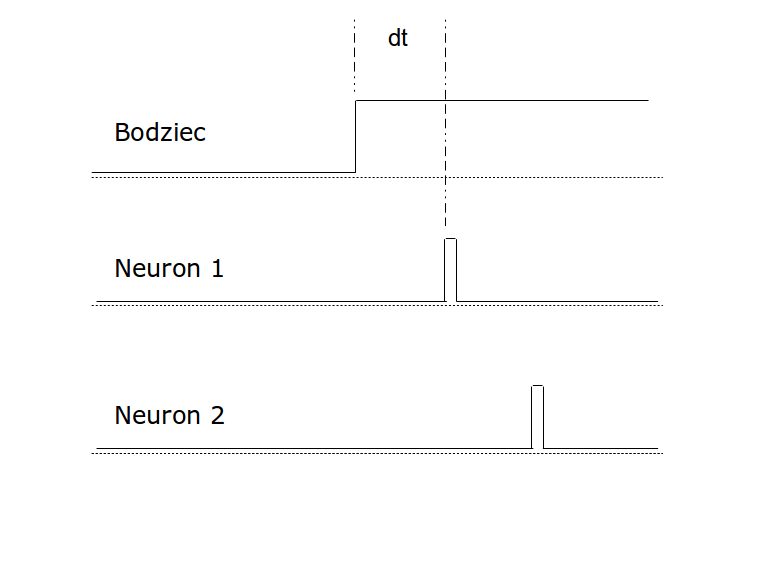
\includegraphics[width=\textwidth/2]{../TimeToFirstSpike.png}
		\caption{Czas najszybszej odpowiedzi}
                \label{fig:TimeToFirstSpike}
	\end{figure}
\subsection{Kodowanie kolejnością przybycia sygnałów}
To podejście wydaje sie być mniej stratne względem poprzedniego, aczkolwiek dalej zapominamy zupełnie o interwałach między impulsami.
Pewne badania wskazują jednak na skuteczność tego modelu w przypadku rozpoznawania statycznych obrazów.
Przykładowy przepływ informacji został pokazany na rys.~\ref{fig:ROC}.
	\begin{figure}[ht]
		\centering
		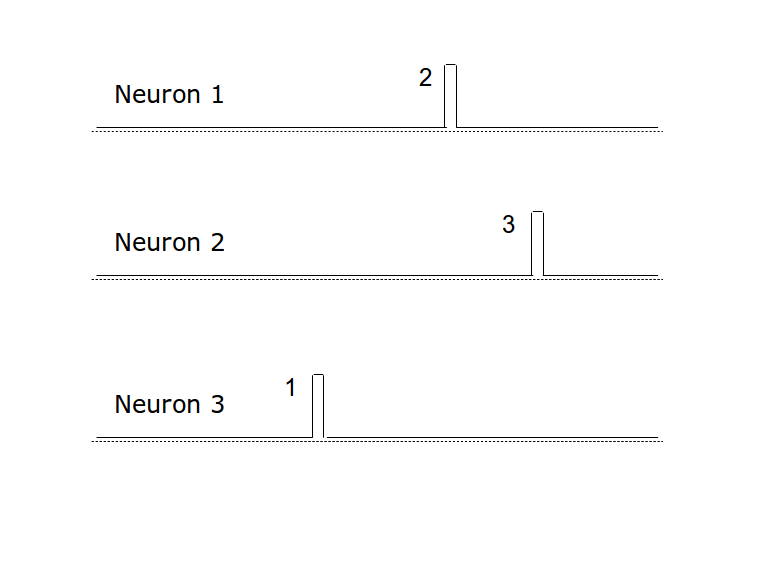
\includegraphics[width=\textwidth/2]{../ROC.png}
		\caption{Kodowanie kolejnością przybycia sygnałów}
                \label{fig:ROC}
	\end{figure}
\subsection{Względne opóźnienie impulsów}
W tym podejściu bierzemy pod uwagę interwały między impulsami, ale nie bierzemy pod uwagę, z którego neuronu wejściowego impulsy pochodziły.
Przykład informacji w tym modelu został przedstawiony na rys.~\ref{fig:Latency}.
	\begin{figure}[ht]
		\centering
		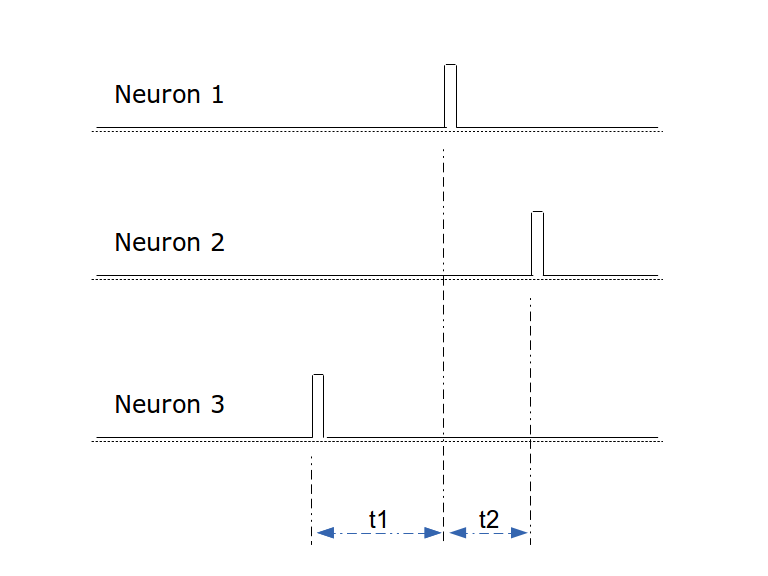
\includegraphics[width=\textwidth/2]{../Latency.png}
		\caption{Względne opóźnienie impulsów}
                \label{fig:Latency}
	\end{figure}
\subsection{Sieć rezonansowa}
W tym podejściu traktujemy neurony jako filtry, które reagują tylko na wybrane częstotliwości. 
Jeden neuron wejściowy przekazuje te same impulsy do kilku neuronów impulsowych. 
W zależności od ich częstotliwości, budzi się tylko jeden neuron. Zostało to zobrazowane na rys.~\ref{fig:ResonantBurst}
	\begin{figure}[ht]
		\centering
		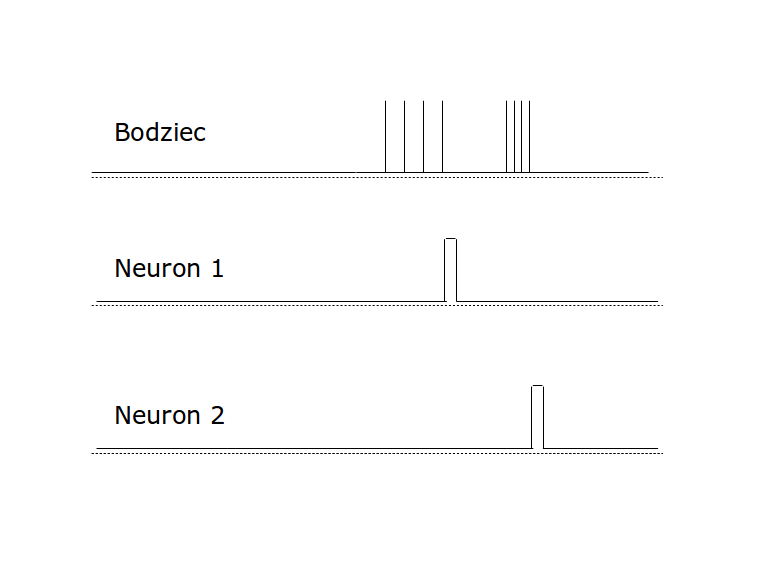
\includegraphics[width=\textwidth/2]{../ResonantBurst.png}
		\caption{Sieć rezonansowa}
                \label{fig:ResonantBurst}
	\end{figure}

\subsection{Kodowanie synchroniczne}
Wartość informacji zależy od tego, na których neuronach impuls pojawił się jednocześnie.
Z badań wynika, że niektóre neurony w ludzkim mózgu są wstanie synchronizować swoje impulsy z odchyleniem mniejszym od 1 ms.
Rys.~\ref{fig:CodingBySynchrony} ilustruje dwie różne wartości informacji w modelu synchronicznym.
	\begin{figure}[ht]
		\centering
		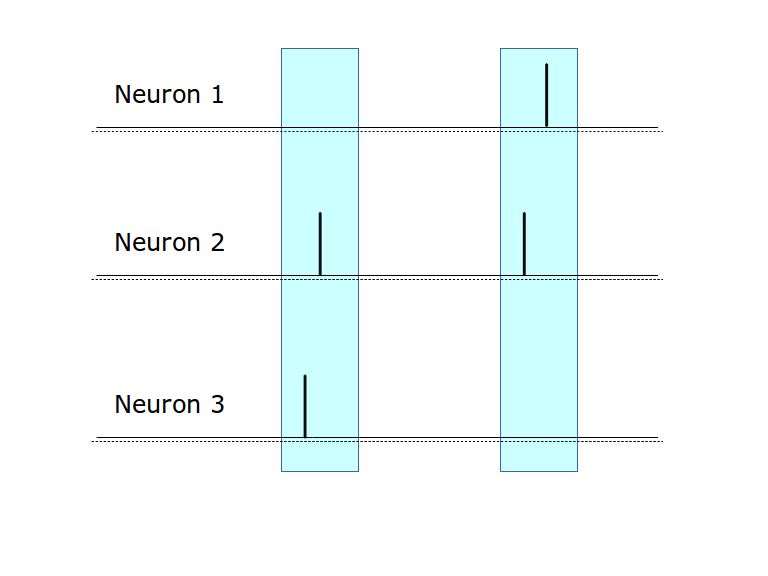
\includegraphics[width=\textwidth/2]{../CodingBySynchrony.png}
		\caption{Kodowanie synchroniczne}
                \label{fig:CodingBySynchrony}
	\end{figure}

\subsection{Kodowanie przez fazę}
W tym podejściu, najbardziej skomplikowanym, informacja zależy od tego, jaka sekwencja impulsów wystąpiła, 
kiedy sygnał referencyjny był w odpowiednim stanie. 
Na rys.~\ref{fig:Phase} przedstawiono takie kodowanie dwóch informacji przy sygnale referencyjnym prostokątnym, 
natomiast częściej stosuje się sygnal sinusoidalny.
	\begin{figure}[ht]
		\centering
		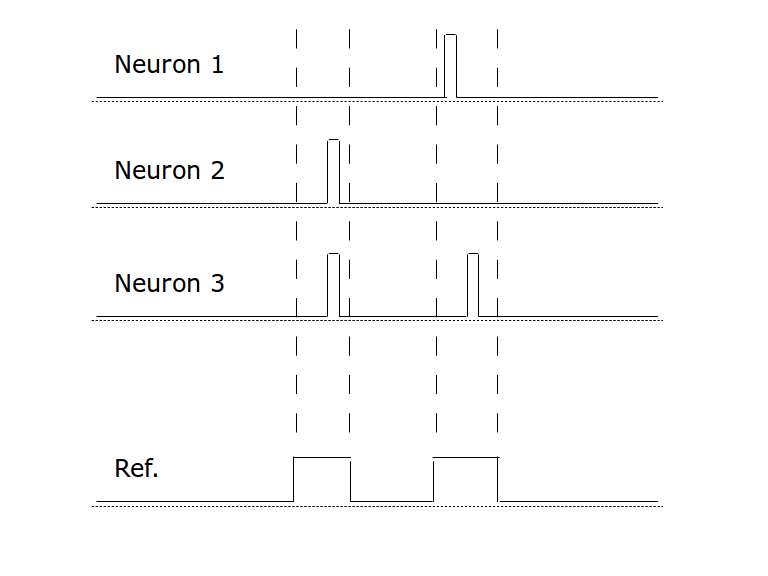
\includegraphics[width=\textwidth/2]{../Phase.png}
		\caption{Kodowanie przez fazę}
                \label{fig:Phase}
	\end{figure}

\section{Topologie}
Posiadając model neuronów i synaps jesteśmy w stanie zdefiniować impulsową sieć neuronową. Typowo, SNN jest traktowana jak skończony graf skierowany (V,E), z V reprezentującymi zbiór neuronów i E - zbiór synaps. Wystrzał neuronów wejściowych jest determinowany na zewnątrz sieci - są one traktowane jako wejście impulsowej sieci neuronowej.

Topologie impulsowych sieci neuronowych są dzielone na trzy kategorie:
1. Sieci w przód (ang. \textit{feedforward}) - przepływ danych z wejść do wyjść jest ściśle jednokierunkowy. Przetwarzanie danych może odbywać w wielu warstwach neuronów, ale nie występują sprzężenia zwrotne. W biologicznych sieciach neuronowych sieci w przód znajdują się głównie w obszarach peryferyjnych. Podobnie, w SNN topologie w przód znajdują głównie zastosowanie w odwzorowywaniu niskopoziomowych zmysłów, takich jak wzrok, węch, dotyk. Sieci w przód są również rozważane w kontekście synchronizacji impulsów, czy przy powiazaniu wzorców przestrzenno-czasowych impulsów.

2. Sieci rekurencyjne - tutaj indywidualne neurony lub populacje tychże komunikują się ze sobą za pomocą wzajemnych połączeń. Wynikiem występowania sprzężeń zwrotnych jest występowanie stanu sieci, które pozwala na traktowanie jej jako system dynamiczny. W konsekwencji sieci rekurencyjne charakteryzują się bogatszą dynamiką i większymi możliwościami obliczeniowymi niż sieci w przód. Niestety, są również trudniejsze w kontroli i uczeniu. Sieci rekurencyjnych używano przy modelowaniu pamięci asocjacyjnej bądź roboczej. Sieci impulsowej z połączeniami rekurencyjnymi były również wykorzystane w analizie zjawisk obserwowanych w mózgu, mających nietrywialny przebieg dynamiczny, wynikający z wzajemnych połączeń między neuronami. 

3. Sieci hybrydowe - grupa ta zawiera sieci, w których niektóre subpopulacje mogą być ściśle w przód, a inne - rekurencyjne. Interakcje między subpopulacjami mogą być jednokierunkowe bądź wzajemne. O ile można wyobrazić sobie wiele potencjalnych architektur takich sieci, skupiono się tu na dwóch najbardziej popularnych i zbadanych klas hybrydowych sieci neuronowych:
\begin{itemize}
\item \textit{Synfire chain} (ang. łańcuch pobudzeń) - ludzka nauka często odbywa się poprzez asocjację dwóch wydarzeń, lub łączenia sygnału i następującej po nim reakcji w pewną relację. Wydarzenia są często odległe w czasie, ale mimo wszystko ludzie są w stanie połączyć je ze sobą, pozwalając na dokładną predykcję odpowiedniego czasu na wykonanie określonej akcji. Łańcuch pobudzeń jest uważany za prawdopodobny mechanizm reprezentujący takie relacje między opóźnionymi względem siebie wydarzeniami. Cechuje się on wielowarstwową architekturą (łańcuch), w którym aktywność impulsów może być propagowana jako synchroniczna fala wystrzałów neuronów ("paczka" impulsów) z jednej warstwy (subpopulacji) łańcucha do kolejnych. Definicja ta sugeruje topologię w przód, niemniej niektóre subpopulacje mogą posiadać wzajemne połącznia.
\item \textit{Obliczenia rezerwuarowe} - jest to obliczeniowa idea, wykorzystująca korzystne cechy sieci rekurencyjnych przy jednoczesnym ominięciu trudności związanych z ich treningiem. W typowej implementacji sieć rezerwuarowa zawiera stałą strukturę rekurencyjną (rezerwuar) i zbiór neuronów wyjściowych, zwanych odczytowymi. Zwykle neurony, odczytowe posiadają wyłącznie jednokierunkowe impulsy z rezerwuaru. Trening sieci polega na uczeniu połączeń między rezerwuarem a warstwą wyjściową. Takie podejście znacznie upraszcza uczenie tych sieci. 
Rezerwuar może być postrzegany jako struktura dokonująca mapowania wejść na wielowymiarowy wektor aktywności neuronów wchodzących w skład sieci. Każdy element tego wektora odzwierciedla wpływ, który poszczególne neurony mogą mieć na elementy wyjściowe. Struktura połączeniowa wewnątrz rezerwuaru jest zwykle losowa i ustalona (niezmienna w trakcie działania). Stabilny stan wewnętrzny rezerwuaru nie jest konieczny do produkowania stabilnych odpowiedzi sieci, gdyż przejściowe stany wewnętrzne mogą być rzutowane na stabilne wyjścia, wykorzystując wysoką wymiarowość systemu dynamicznego. Ponadto, stan rezerwuaru i przejścia pomiędzy nimi nie muszą być dostosowywane do konkretnych zadań. Oznacza to, że ta sama, dostatecznie duży, generyczny rezerwuar może być wykorzystywany przy zadaniach obliczeniowych różnego rodzaju. Sieci rezerwuarowe były z sukcesem wykorzystywane do takich zadań jak rozpoznawanie mowy ludzkiej, predykcji ruchu czy jego kontroli.
\end{itemize}
\section{Uczenie}
Plastyczność synaptyczna odnosi się do zdolności połączeń synaptycznych do zmiany swojej przewodności, która jest uważana za podstawowy mechanizm uczenia i pamięci w biologicznych sieciach neuronowych. Współistnieją ze sobą różnorakie formy plastyczności synaptycznej. Różnią się one przede wszystkim na skali czasu: niektóre procesy wygasają w czasie rzędu 10-100 ms, a inne - np. długotrwała depresja (ang. \textbf{LTD} - \textit{Long Term Depression}) utrzymują się przez wiele godzin, dni lub dłużej. Procesy plastyczności różnią się także warunkami koniecznymi do indukcji. Niektóre zależą wyłącznie od historii presynaptycznej stymulacji, niezależnie od postsynaptycznych odpowiedzi. Inne formy plastyczności zależą od współwystępowania odpowiednich pre- i postsynaptycznej odpowiedzi, na czasową kolejność pre- i postsynaptycznych impulsów oraz prawdopodobnie innych czynników, takich jak koncentracja określonych substancji chemicznych. 
W niniejszej pracy dyskutowane są różne modele uczenia impulsowych sieci neuronowych które wykorzystują plastyczność synaptyczną opartą na zależnościach czasowych impulsów.
\subsection{Uczenie bez nadzoru}
W 1949 roku Donald Hebb po raz pierwszy odpowiedział na pytanie w jaki sposób synapsy zmieniają swe wagi tak, czy przechowywać informacje. Matematycznie jego idea może być wyrażona jako: $\Delta w_{ji} \infty \mu_j \mu_i$, gdzie $\Delta w_{ji}$ odnosi się do zmiany siły synaptycznego połączenia $w_{ji}$ pomiędzy presynaptycznym neuronem $i$, a postsynaptyczną komórką $j$; $\mu_i, \mu_j$ wyrażają aktywność tych neuronów. Zgodnie z formułą Hebba, połączenie $w_{ji}$ jest wzmacniane, gdy neurony $i$ i $j$ są jednocześnie aktywne. Równanie to nie opisywało synaptycznej depresji. Jedynie późniejsze badania teoretyczne i eksperymentalne pomogły ustalić warunki, przy których mogło do niej dojść.
Modyfikując przewodności synaptyczne, procesy Hebba prowadzą do reorganizacji połączeń wewnątrz sieci neuronowej i przy pewnych warunkach mogą tworzyć nowe funkcje, takie jak grupowanie wejść, rozpoznawanie wzorców, redukcję wymiarowości, formację pamięci asocjacyjnych lub samoorganizujących map. Wytworzenie tych własciwości poprzez process Hebba jest powszechnie znany jako uczenie bez nadzoru, gdyż nie stawia się sieci żadnego konkretnego celu uczenia i nie jest potrzebna żadna korelacja w procesie tworzenia funkcji wewnątrz sieci. 
Wyrażenia $\mu_i, \mu_j$ w formule Hebba tradycyjnie były interpretowane jako częstości impulsów neuronów. Niedawne odkrycia z dziedziny neurofizjologii sugerują jednak, że plastyczność Hebba może być również zmieniana czasem wystąpienia poszczególnych impulsów. Co więcej, dowody z komórek hippokampa wskazują, że kolejność wystąpienia impulsów pre- i postsynaptycznych mogą indukować różne procesy Hebba. W jednym eksperymencie modyfikowano relatywny czas między dotarciem presynaptycznego impulsów w synapsie a postsynaptycznym potencjałem czynnościowym \cite{Markram97}. Zaobserwowano, że zmiana w przewodności synaptycznej po kilku iteracjach eksperymentu była funkcją relatywnych różnic w czasach impulsów. Generalnie rzecz biorąc, presynaptyczne impulsy występujące przed postsynaptycznymi indukowały wzmocnienie, podczas gdy odwrotna kolejność powodowała depresję synaptyczną. Zjawisko to nazwano plastycznością zależną od czasu impulsów (ang. \textbf{STDP} - \textit{Spike timing Dependent Plasticity}). W niektórych synapsach obserwowano odwrotne zjawisko, teraz znane jako Anty-STDP.
Co ciekawe, zależność plastyczności synaptycznej od czasu występowania impulsów była przewidziana teoretycznie. Zaproponowano model, wyrażony jako: $\frac{d}{dt} w_{ji}(t) = a_0 + a_1 S_i(t) + a_2 S_j(t) + a_3 S_i(t) \overline{S_j}(t) + a_4 \overline{S_i}(t)S_j(t)$, gdzie $w_{ji}(t)$ jest przewodnością połączenia synaptycznego między neuronem $i$ oraz $j$; $S_i(t)$ i $S_j(t)$ są paczkami impulsów pre- i postsynaptycznych, a $\overline{S_i}(t)$ i $\overline{S_j}(t)$ to wersje $S_i(t)$ i $S_j(t)$, po filtracji dolnoprzepustowej. Współczynniki $a_0,...,a_4$ są stałymi kontrolującymi szybkość zmian przewodności synaptycznej. 
Powyższe równanie zakłada, że prócz spadku niezależnego od poziomu aktywności ($a_0$) i współczynników Hebba $a_3 S_i(t)\overline{S_j}(t), a_4 \overline{S_i}(t) S_j(t)$, zmiany w potencjale synaptycznym mogą wynikać z indywidualnych impulsów po stronie pre- lub postsynaptycznej, nawet w przypadku braku reakcji po drugiej stronie synapsy. Odpowiednio dobierając współczynniki powyższego równania, jesteśmy w stanie zamodelować proces STDP, Anty-STDP lub inne.

\subsection{Uczenie z nadzorem}
Uczenie z nadzorem jest wykorzystywane w sztucznych sieciach neuronowych od początkowych lat teorii obliczeń neuronowych. Niedawno zgromadzono więcej dowodów na to, że takie uczenie jest również wykorzystywane przez mózg \cite{Knudsen94}. Najbardziej udokumentowanym zjawiskiem tego rodzaju jest uczenie centralnego układu nerwowego, a zatem związane z kontrolą ruchową. W szczególności, uczenie z nauczycielem jest najprawdopodobniej wykorzystywane przez ośrodki ruchowe do formowania wewnętrznych reprezentacji ciała i otoczenia.
Sygnały uczące mają formę szkieletów aktywności, które mają zostać zreprodukowane. W układzie nerwowym sygnały te są dostarczane do modułów uczących poprzez zmysły lub od innych neuronowych struktur nadzorczych. Nie wiemy jednak jaka jest dokładna reprezentacja neuronowych sygnałów uczących oraz jak neurony biologiczne uczą się generować zadane wyjścia na ich podstawie. 
Spośród niewielu rozpoznanych metod uczenia z nauczycielem sieci impulsowych, uczenie Hebba z nadzorem (ang. \textbf{SHL} - \textit{Supervised Hebbian Learning}) oferuje prawdopodobnie najbardziej oczywiste rozwiązanie dla implementacji nadzoru w sposób realistyczny biologicznie. Zgodnie z tym podejściem impulsowy proces Hebba jest nadzorowany przez dodatkowy sygnał uczący, który wzmacnia neuron postsynaptyczny, by wystrzeliwał w zadanych momentach czasowych i pozostawał uśpiony w pozostałych. Sygnał uczący jest zazwyczaj transmitowany do neuronu w formie ładunków synaptycznych lub ładunków wstrzykiwanych wewnątrzkomórkowo. Podczas badań metody dostrzeżono jej pewne ograniczenie: ponieważ ładunki uczące tłumią wszystkie niepożądane wystrzały w trakcie treningu, jedyne korelacja między aktywnością pre- i postsynaptyczną zachodzi w okolicy zadanych czasów wystrzałów. W pozostałym czasie, nie ma korelacji, nie ma mechanizmu osłabiającego wagi synaptycznych, które powodują wystrzał neuronu w niepożądanych okresach czasu. Stabilne rozwiązania w SHL mogą zostać osiągnięte wyłącznie przy dodatkowych założeniach (regułach uczących). 
Problemy te były zaadresowane w algorytmie ReSuMe \cite{Ponulak2011}. Podobnie do SHL, wykorzystuje on procesy Hebba, lecz sygnał uczący powinien mieć jak najmnieszy wpływ na postsynaptyczny potencjał somatyczny membrany. W ReSuMe, waga synaptyczna jest modyfikowana zgodnie z poniższym równaniem:
 
$\frac{d}{dt} w_{ji}(t) = a \left[S_d(t) - S_j(t) \right] \overline{S_i}(t)$, gdzie a - szybkość uczenia, $S_d$ - referencyjny ciąg impulsów, $S_j$ - odpowiedź sieci, $\overline{S_i}(t)$ - ciąg impulsów wejściowych, po użyciu filtra dolnoprzepustowego.

Równanie opisuje ReSuMe jako metodę łączącą dwa procesy Hebba: pierwszego zdefiniowanego na zadanej i presynaptycznej paczce impulsów, oraz drugiego, anty-Hebbowego, zdefiniowanego na paczkach impulsów pre- i postsynaptycznych. Warto zauważyć, że prawa strona równania ma podobną postać do znanej nam reguły Widrowa-Hoffa.

O ile przedstawione wyżej metody z powodzeniem uczą sieci jednowarstwowe, bardziej pożądane są sposoby uczenia sieci wielowarstwowych i rekurencyjnych, z uwagi na ich zwiększone możliwości obliczeniowe. Niestety, implementacja algorytmu wstecznej propagacji dla sieci impulsowych jest utrudniona, ze względu na złożoną i ich często nieciągłą dynamikę. Pierwszy zaproponowany algorytm, zwany SpikeProp, wykorzystał powyższą, przy jednym poważnym ograniczeniu - każdy neuron mógł wystrzelić tylko raz w trakcie okresu uczenia. Z biegiem czasu algorytm został jednak udoskonalony i z powodzeniem jest wykorzystywany w praktyce.

\subsection{Uczenie w obecności sygnału nagrody} 

Zwierzęta w przyrodzie uczą się nowych zachowań nie tylko w obecności bezpośrednich instrukcji, lecz częściej rozważając dostępne opcje w obecności sygnałów nagrody. W procesie prób i błędów najlepsze wybory są wzmacniane, a złe - osłabiane sygnałami kary. Taki sposób uczenia został już pomyślnie wykorzystany w dziedzinie machine learning. Dostrzeżono również, że w podobny sposób uczy się ośrodek dopaminergiczny. Ściślej, koncentracja dopaminy, neuromodulatora emitowanego przez komórki dopaminergiczne, kontroluje procesy plastyczności w wielu obszarach mózgu. 

Na postawie powyższych obserwacji powstało kilka metod uczenia w obecności sygnału nagrody. Wiele z nich może było opisanych przez następującą, generyczną formułę: 
$\frac{d}{dt}w_{i,j}(t) = c_{ji}(t)d(t)$, gdzie $w_{ji}$ oznacza wagę połączenia synaptycznego między neuronem $i$ oraz $j$, $c_{ji}(t)$ to podatność tej synapsy na zmiany.

Zaproponowane modele łączące teorię nauki przy udziale nagrody / kary i plastyczność synaptyczną opartą na kodowaniu impulsowym zostały wykorzystane do wyjaśnienia wielu zjawisk zaobserwowanych eksperymentalnie. Impulsowe sieci neuronowe zostały również z powodzeniem wykorzystane do rozwiązania szeregu zadań inżynierskich. 

\section{SNN a kora wzrokowa}

System wizyjny u ssaków jest dużo bardziej skomplikowany, w porównaniu do przetwarzania obrazów zestawem iloczynów skalarnych.
Neurobiolodzy nie są nawet blisko zrozumienia wszystkich operacji,
oczywiste jest, że zwykłe algorytmy informatyczne używane do rozpoznawania obrazów nie są w stanie odwzorować układu wzrokowego.
Wejściem obrazu jest oczywiście oko. 
Receptory siatkówki z tyłu gałki są nierównomiernie rozłożone i wrażliwe są na różne niesione informacje.
Inne są wrażliwe na ruch, kolor, nasycenie. Jednocześnie jednak są ze sobą powiązane.
Kiedy receptor dostaje odpowiednią informację, zmienia zachowanie innych, otaczających receptorów.
Operacje matematyczne są więc przeprowadzone jeszcze zanim obraz opuści oko.


Oko dodatkowo dostaje informacje zwrotne. 
Ludzie nie patrzą w jeden punkt, zbieramy informację zgodnie z kontekstem całego obrazu.
Dodatkowo, to sprzężenie zwrotne oddziałowuje na wyjście z receptorów.

Gdy informacje obrazu opuszczają oko, trafiają do kory wzrokowej.
Tutaj obraz jest analizowany przez mózg.
Badania nad korą wzrokową kota i świnki morskiej są podstawą modeli użytych w tym rozdziale.
Chociaż te modele są dużym krokiem w stronę symulowania systemu wizyjnego ssaków,
to wciąz jest to bardzo uproszczony model, bardzo skomplikowanego systemu.
Intensywne badania trwają by móc całkowicie zrozumieć cały proces.
Obecnie, algorytmy wypadają diametralnie słabo w porównaniu z rozpoznawaniem obrazu u człowieka.
Powód jest oczywisty, są one bardzo proste w porównaiu z rzeczywistym biologicznym systemem.

Emulowanie pewnych systemów biologicznych jest konieczne, by zwiększyć zaawansowanie systemów komputerowych.
Jednym z ważnych krokół jest zamodelowanie procesów przeprowadzanych w korze wzrokowej.
Zaczynają być zrozumiałe, jednak wciąż istnieją debaty na ich temat.
Procesy te są bardzo potężne i zrozumienie ich może prowadzić do powstania nowych narzędzi służących do rozpoznawania obrazów.

\subsection{Kora wzrokowa}
W podrozdziale będzie rozważana teoria i aplikacja dwóch modelu korowych:
\begin{itemize}
	\item PCNN (pulse coupled neural network) - Model sieci impulsowych
	\item ICM (intersecting cortical model)
\end{itemize}

Modele te są oparte na biologicznych modelach kory wzrokowej.
Jest więc konieczne, by zrobić przegląd algorytmów, 
które mocno wpłynęły na opracowanie modeli PCNN i ICM

Niezależnie od stopnia odwzorowania, czy podobieństwa do biologicznego modelu,
algorytmy użyte jako modele korowe są przydatne.
\begin{figure}[H]
 
	\centering
	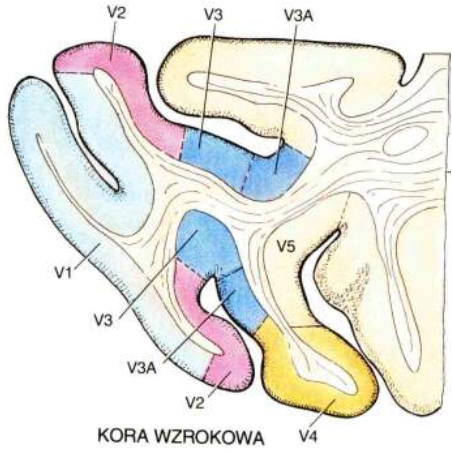
\includegraphics[width=\textwidth/2]{KoraWzrokowa.png}
	\caption{Kora wzrokowa} \label{fig:Korawzrokowa}
\end{figure} 
\begin{figure}[ht]
	\centering
	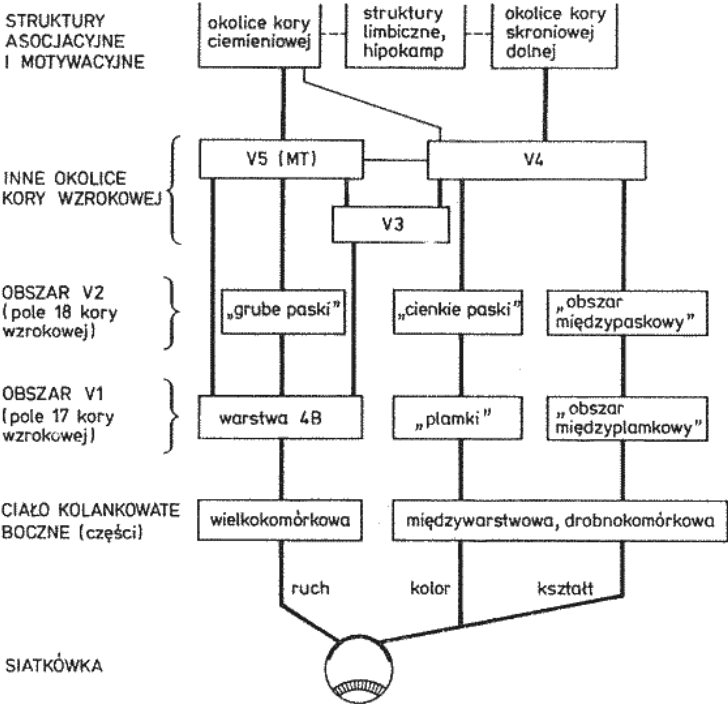
\includegraphics[width=\textwidth*4/5]{ModelKory.png}
	\caption{Model systemu wizyjnego} \label{fig:Modelkory}
\end{figure}
\ref{fig:Korawzrokowa} przedstawia korę wzrokową, a \ref{fig:Modelkory} model systemu. Istnieją dwa w znacznej mierze rozdzielone szlaki przetwarzania informacji wzrokowej, biegnącej już od oka:
\begin{itemize}
\item Wielkoziarniste komórki $PA$ siatkówki, 3 typy stożków fotorecepcyjnych, duże pola recepcyjne, szybko przewodzące aksony, pobudzenie dla światła w szerokim paśmie.
\item Drobnoziarniste komórki $PB$, 1 lub 2 typy stożków fotorecepcyjnych, małe pola recepcyjne, wolno przewodzące aksony, rozpoznają opozycje barw.
\end{itemize}
\textbf{Szlak wielkokomórkowy}: biegnie do dwóch wielkokomórkowych warstw LGN (jest w nich ok. 100.000 komórek), charakteryzuje go niska rozdzielczość przestrzenna, wysoka wrażliwość na kontrast, szybkie przesyłanie sygnałów, bez informacji o kolorze.
Ta informacja trafia przez płat potyliczny szlakiem grzebietowym do kory ciemieniowej.
Dochodzi do warstwy 4B w V1, stąd do grubych ciemnych pasków obszaru V2, analizuje informację o ruchu obiektu.
\begin{itemize}
\item W V1, warstwa $4B => V5$, lokalizacja w polu widzenia, ruch.
V5 pobudza płat ciemieniowy, PPC (tylna kora ciemieniowa), obszar 7 i 5; umożliwia to orientację przestrzenną, postrzeganie głębi i ruchu, połączenie z wzgórkami czworaczymi (orientacja oczu).
\end{itemize}
\textbf{Szlak drobnokomórkowy} ma 4 drobnoziarniste warstwy i 10 razy więcej komórek niż wielkokomórkowy w LGN.
Duża rozdzielczość przestrzenna, kolor, wolniejszy przesył informacji, niska wrażliwość na kontrast.
Ta informacja trafia szlakiem brzusznym do kory dolnoskroniowej.
\begin{itemize}
\item $V1 => V2$ obszar międzyplamkowy, reaguje na orientację linii, daje dużą ostrość widzenia, bez koloru.
\item $V1 => V3$ obszar plamkowy, reaguje na kształty, reakcja na kolor w neuronach w ciemnych prążkach V3.
\item $V2 => V4$, główny obszar analizy koloru, informacja dochodzi do kory dolnoskroniowej (IT).
Obszar IT w płacie dolnoskroniowym ma neurony reagujące na złożone obiekty. 
\end{itemize}



\subsection{Model Hodgkina-Huxleya}
Badania na temat kory wzrokowej ssaków przedstawione ponad pół wieku w pracy Hodgkina i Huxleya
zdefiniowały system opisujący potencjał błonowy następująco:
$$I=m^3 hG_{Na} (E-E_{Na}) + n^4G_K(E-E_K)+G_L(E-E_L) $$
\begin{itemize}
\item $I$ -- prąd jonowy
\item $m$ -- prawdopodobieństwo otwarcia kanału
\item $G$ -- konduktancja (dla sodu, potasu i przenikania)
\item $E$ -- Potencjał
\end{itemize}
Prawdopodobieństwo pisane następująco:
$$\frac{dm}{dt}=a_m(1-m)-b_mm$$
$a_m$ jest współczynnikiem bramek nie otwartych, a $b_m$ jest współczynnikiem aktywacji bramek.

Ważność korowego systemu jest taka, że neurony są opisane jako równanie różniczkowe.
Prąd jest zależny od współczynników zmian poszczególnych chemicznych elementów.
Dynamika neuronu jest opisana jako proces oscylacyjny.
\subsection{Model Fitzhugh-Nagumo}
Zachowanie neurona w pracy popełnionej przez Fitzhugh i Nagumo kilka lat później, 
zostało opisane jako oscylator van der Pola.
Ten model jest opisany w różnoraki sposób, ale częścią wspólną zawsze jest sparowany oscylator dla każdego neuronu.
W swojej pracy podają przykład, gdzie $x$ jest pobudzeniem, a $y$ przywróceniem. 
$$\varepsilon\frac{dx}{dt}=-y-g(x)+I$$
$$\frac{dy}{dt}=x-by,$$

Gdzie:
\begin{itemize}
\item $g(x) = x (x-a) (x-1)$
\item $0<a<1$ 
\item $I$ jest prądem wejściowym 
\item $\varepsilon\ll1$
\end{itemize}
\ref{fig:FitzhughNagumoequation} ukazuje system oscylacyjny opisany równaniami Fitzhugh-Nagumo.
Te równania opisują prosty system i bardzo proste sumulacje potrafią zaprezentować różne charakterystyki systemu.
Dla przypadku $\varepsilon=0.3$, $a=0.3$, $b=0.3$ i $I=1$ można uzyskać zachowanie jak na rysunku \ref{fig:FitzhughNagumoequation}.
Po zmianie wartości $b=0.6$ można wygenerować system przedstawiony na rysunku \ref{fig:FitzhughNagumoequation2}.
Model zaprezentowany przez Fitzhugh i Nagumo jest ważny z tego względu,
że opisuje neurony w taki sposób, który może zostać użyty w wielu różnych biologicznych modelach.
Każdy neuron reprezentuje dwa oscylatore połączone z innymi neuronami.
\begin{figure}[ht]
	\centering
	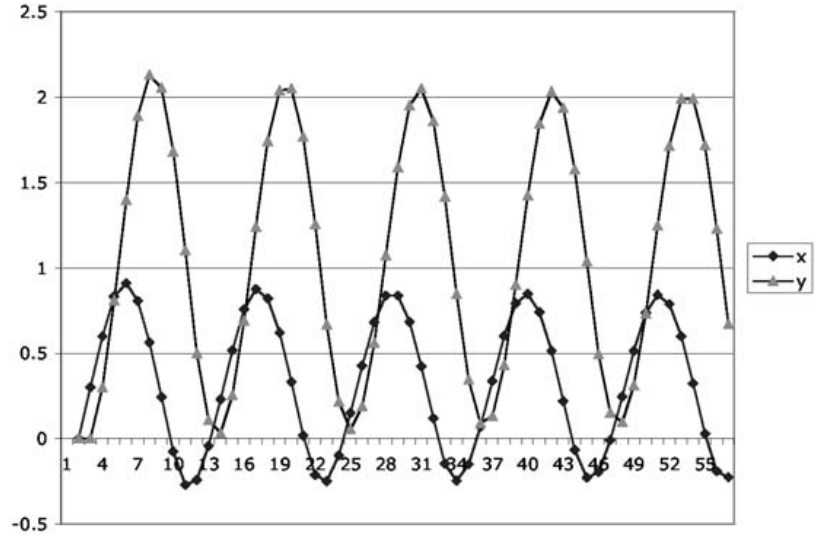
\includegraphics[width=\textwidth*4/5]{FitzhughNagumoequation.png}
	\caption{System oscylacyjny opisany równaniami Fitzhugh-Nagumo} \label{fig:FitzhughNagumoequation}
\end{figure}
\begin{figure}[ht]
	\centering
	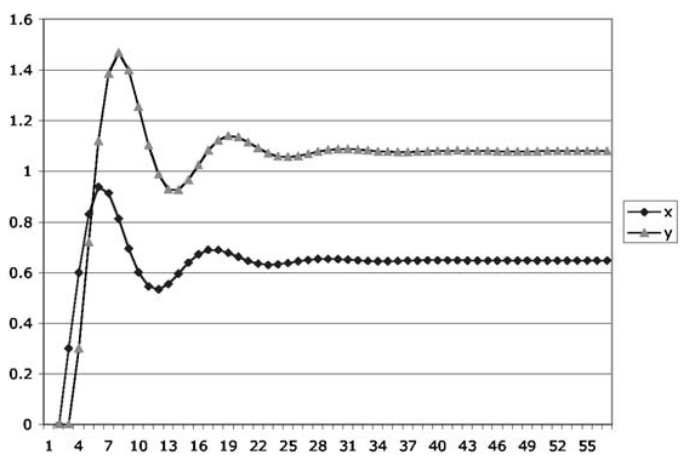
\includegraphics[width=\textwidth*4/5]{FitzhughNagumoequation2.png}
	\caption{System oscylacyjny opisany równaniami Fitzhugh-Nagumo} \label{fig:FitzhughNagumoequation2}
\end{figure}
\subsection{Model Eckhorna}
\begin{figure}[H]
	\centering
	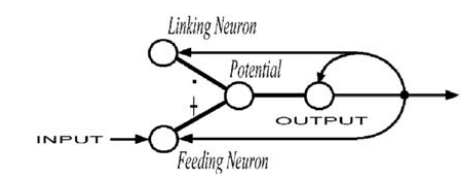
\includegraphics[width=\textwidth*3/5]{../EckhornNeuron.png}
	\caption{Neuron typu Eckhorna } \label{fig:EckhornNeuron}
\end{figure}

Eckhorn wprowadził model oprarty na korze wzrokowej kota.
Jego schemat przedstawiony na rysunku \ref{fig:EckhornNeuron}.
Komunikacja pomiędzy neuronami została pokazana na rysunku \ref{fig:PCNNNeuron}.
Sieć składa się z warstwy neuronów połączonych ze sobą dwoma rodzajami sprzężeń zwrotnych:
\begin{itemize}
\item feeding(F)
\item linking (L)
\end{itemize}
Rezultatem porównania jest napięcie membrany, $U_m$, które jest następnie porównane do lokalnego progu, $\Phi$

Model Eckhorna prezentują następujące równania:
$$U_{m,k} (t)=F_k(t)[1+L_k (t)]$$
$$F_k(t)=\sum\limits_{i=1}^N [\omega_{ki}^f Y_i(t)+S_k(t)+N_k(t)]\bigotimes I (V^a, \tau^a,t)$$
$$L_k(t)=\sum\limits_{i=1}^N [\omega_{ki}^l Y_i(t)+N_k(t)]\bigotimes I (V^l, \tau^l,t)$$
$$ \mathbf{Y_k(t)} =
\left\{ \begin{array}{ll}
1 & \textrm{dla $U_{m,k}(t)\geq \phi_k(t)$}\\ 
0 & \textrm{pozostałe przypadki}
\end{array} \right.$$

W przypadku ogólnym
$$X(t)=Z(t)\bigotimes I(v,\tau,t)$$

da się przedstawić jako:
$$X[n] = X[n-1]e^{\frac{-t}{\tau}} + V Z[n] $$

$N$ jest liczbą neuronów, $\omega$ wagą synaptyczną, $Y$ wyjściem binarnym, $S$ pobudzeniem zewnętrznym.
Typowe zakresy wartości wynoszą $\tau^a=[10,15]$, $\tau^l=[0.1, 1.0]$, $\tau_s=[5,7]$, 
$V^a=0.5$, $V^l=[5,30]$, $V^s=[50,70]$, $\phi_o=[0.5,1.8]$.

\begin{figure}[ht]
	\centering
	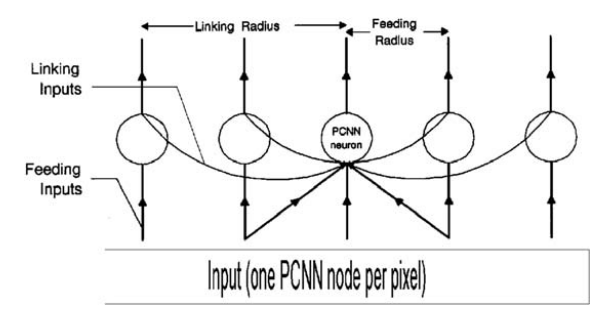
\includegraphics[width=\textwidth*4/5]{../PCNN.png}
	\caption{Neuron PCNN} \label{fig:PCNNNeuron}
\end{figure}
\subsection{Model Rybaka}
Elementem badań Rybaka była kora wzrokowa świnki morskiej i odkrył podobne zależności, co w modelu Eckhorna.
Równania są różne, natomiast samo zachowanie neuronu jest całkiem podobne.
Neuron Rybaka ma 2 porównania $X$ i $Z$. 
Następuje ich interakcja z pobudzeniem, $S$ : 
$$X_{ij}^S=F^S\bigotimes||S_{ij}||$$
$$X_{ij}^I=F^I\bigotimes||Z_{ij}||$$
$$Z_{ij}=f\left\{\sum X_{ij}^S - \left( \frac{1}{\tau p+1} \right) X_{ij}^I -h \right\}$$

Gdzie $F^S$ są połączeniami centrum/otoczenie.
$F^I$ to lokalne połączenia kierunkowe, $\tau$ to stała czasowa i $h$ jest globalnym inhibitorem.
$f{}$ jest funkcją progowania.
\subsection{Model Parodi}
Wciąż istnieje małe podobieństwo do rzeczywistego modelu kory wzrokowej.
Parodi zaproponował alternatywę dla modelu Eckhorna. 
Argumentami przeciwko modelowi Eckhorna były m.in. brak synchronizacji w neuronach,
nieporządane podobne wyjścia dla elementów poruszających się i stacjonarnych, 
czy to, że modulacje neuronu w sprzężeniu L były znacznie wyższe niż przewidywał to model Eckhorna.

Parodi zaproponował więc model alternatywny, zawierając w nim opóźnenia związane z połączeniami synaptycznymi
i wprowadził reset neuronu \textit{en masse}.
$$\frac{\partial V(x,y,t)}{\partial t} = - \frac{V(x,y,t)}{\tau} 
+ D\Delta ^2V(x,y,u)+h(x,y,t)$$

$V_i$ jest potencjałem $i$--tego neuronu, $D$ jest dyfuzją $(D = \frac{a^2}{C} R_c)$,
$R_c$ jest rezystancją sprzężeniową neuronu, $t= C R_l$, $R_1$ jest rezystancją upływową.
$R_c^-1<R_l^-1$

$$h_i(t)=\sum\limits_j \omega_{ij} \delta (t-t_j^s - \tau_{ij})$$
\subsection{Podsumowanie}
Biologiczne modele kory wzrokowej przedstawiają każdy neuron jako parę oscylatorów połączonych z innymi neuronami.
To różni się znacząco od tradycyjnego cyfrowego przetwarzania obrazów opartych głównie o operacje matematyczne pierwszego rzędu.
Stworzenie odpowiednio potężnych algorytmów będzie wymagało w przyszłości użycia odpowiednio potężnych maszyn.
Możliwe, że w przyszłości modele oparte o korę wzrokową ssaków będą zaimplementowane w przetwarzaniu obrazów.

\section{Zastosowania SNN}

Zastosowania impulsowych sieci neuronowych zależą od zastosowanych metod uczenia. Jak zostało już napisane, wyróżnia się trzy podstawowe rodzaje uczenia sieci tego typu: uczenie z nauczycielem (\emph{supervised learning}), uczenie bez nauczyciela (\emph{unsupervised learning}) oraz uczenie metodą reinforcement learning. 

W przypadku uczenia bez nauczyciela, do głównych zastosowań sieci impulsowych, opisywanych w pracy~\cite{Ponulak2011} należą:

\begin{itemize}

\item Klasyfikacja danych
\item Rozpoznawanie obrazów, zapachów
\item Nawigacja przestrzenna, tworzenia map środowiska i jego eksploracja
\item Samoorganizujące się mapy (\emph{Self Organizing Maps})
\item Rozpoznawanie szeregów czasowych
\item Pamięci asocjacyjne
\item Wyznaczanie głównych składowych ciągów impulsów

\end{itemize}

Impulsowe sieci neuronowe uczone z nauczycielem znajdują zastosowanie w:

\begin{itemize}

\item Sterowaniu silnikami (serwomechanizmy) i planowaniu ruchu
\item Klasyfikacji danych
\item Podejmowanie decyzji, szczególnie w kontekście rynków finansowych

\end{itemize}

Sieci uczone metodami reinforcement learning mogą zostać użyte do:

\begin{itemize}

\item Nawigacji przestrzennej i planowania ruchu
\item Podejmowania decyzji

\end{itemize}

Wybrane aplikacje opisane zostały dokładniej w prezentacji. 


\subsection{SpiNNaker -- neuromorficzny superkomputer}

Symulacja złożonych sieci impulsowych w czasie rzeczywistym wymaga znacznej mocy obliczeniowej, wielokrotnie przekraczającej możliwości współczesnych komputerów. Jednym z projektów mających na celu implementację bardzo złożonych sieci impulsowych (o liczbie neuronów wynoszącej około 1\% wszystkich neuronów zawartych w ludzkim mózgu) jest SpiNNaker, prowadzony na Manchester University w Wielkiej Brytanii. System ten ma stać się docelowo platformą do badania bardzo wielu algorytmów oraz typów sieci, co będzie możliwe ze względu na jego rekonfigurowalną strukturę.

Po stronie sprzętowej system (w ostatecznej wersji) składać się będzie z 65536 identycznych, 18 rdzeniowych procesorów. Każdy rdzeń ARM968 taktowany jest zegarem 200 MHz. Procesory te wytwarzane są w stosunkowo starym procesie technologicznych 130 nm, co wpływa niekorzystnie na ich pobór energii. Możliwości pojedynczego rdzenia w zakresie symulacji sieci neuronowych nie są wielkie -- jest on w stanie modelować działanie około 1000 neuronów. Jeżeli jednak uwzględni się ogromną ich liczbę w całym systemie (1178648), możliwe stanie się wykonywanie nawet bardzo złożonych sieci w czasie rzeczywistym. 

Komunikacja pomiędzy rdzeniami realizowana jest w sposób w pełni cyfrowy. Dane przesyłane są w 40 lub 72 bitowych pakietach, w których aż 32 bity użyte są do określenia neuronu źródłowego. Każdy z procesorów przyłączony jest do sześciu sąsiednich układów, jednak możliwa jest realizacja dowolnych połączeń na poziomie sieci neuronowej.




%%%%%%%%%%%%%%%%%%%%%%%%%%%%%%%%%%%%%%%%%%%%%%%%%%%%%%%%%%%%%%%%%%%%%%%%%

\newpage{}

\listoffigures

\newpage{}

\nocite{*}
\bibliographystyle{plain}
\bibliography{../bibliografia}

\end{document}

